%Chapter5 角动量理论与自旋
\begin{introduction}
    \item 角动量与旋转不变性 \ref{section5.2}
    \item 角动量的代数求解  \ref{section5.3}
    \item 电子的自旋角动量 \ref{section5:spin}
    \item 角动量的耦合 \ref{section5:coupling}
\end{introduction}
%5.1节角动量概述
\section{角动量概述}
本节我们来研究量子力学的角动量,这里涉及的领域非常重要,很多结果已经渗透到物理学的方方面面,比如:原子光谱、分子光谱;基本粒子的自旋与磁性等。在本章涉及的角动量大体分为两种,一种角动量是与经典角动量对应的。比如在经典力学中,如果一个质量为$m$的质点$P$处于有心势场\footnote{有心势场指的是势能函数只和$P$与空间中给定一点(我们设为原点$O$)的距离有关}中,则$P$点受到的力总是指向$O$,因而该点相对于$O$点的力矩为0,于是满足角动量定理:

\begin{equation}
     \frac{d}{dt}L=0
\end{equation}

而所有这些性质在量子力学中都有对应,我们在中会详细的说明。而另一方面,在20世纪发现了许多违背当时理论的实验现象,比如$Stern-Galach$实验、$Zeeman$效应等,这些现象用经典对应的角动量理论是不能解释的,因此科学家认为,一定还存在一种“典型量子化”的角动量,也就是说,这种角动量只和粒子的内禀性质有关。于是我们称第一种情况下的角动量为轨道角动量,其对应的观察算符用$\hat{L}$表示;而后一种典型量子化的角动量我们统称为自旋角动量,我们用符号$\hat{S}$表示。对于基本粒子组成的体系来说,各个轨道角动量$\hat{L_i}$之间相互组合,并且同时与各个自旋角动量相互组合构成了总角动量$\hat{J}$。本章首先讨论角动量$\hat{J}$的普遍性质,随后进一步讨论自旋的性质,最后探讨角动量的耦合作用。

\begin{remark}
\underline{\textbf{如果没有特别说明是哪种角动量,我们统一用$\hat{J}$表示任意的角动量。}}
\end{remark}
%5.2节 角动量的普遍性质
\section{角动量的普遍性质}
本节的目标是得到角动量的普遍性质。我们首先从经典力学的角动量出发,通过正则量子化得到轨道角动量$\hat{L}$的对易关系;随后通过了解角动量的本质是空间转动群的生成元,将角动量的对易关系扩展到一般的角动量$\hat{J}$上,最后利用对易关系以及谐振子中提到的代数方法得到角动量的本征值与本征函数性质。
    \subsection{轨道角动量的性质}
    在经典力学中,我们知道角动量的定义为:
    \begin{equation}\label{equ:5.2}
    L=r\times p
    \end{equation}

    在高等数学中,我们已经知道了叉乘的计算方法,于是我们可以将式\ref{equ:5.2}展开成分量形式:
    \begin{equation}
        L=(L_x,L_y,L_z)=
        \begin{vmatrix}
        e_x & e_y & e_z\\
        x & y & z\\
        p_x & p_y & p_z
        \end{vmatrix}
         =(yp_z-zp_y,zp_x-xp_z,xp_y-yp_z)
    \end{equation}

    观察轨道角动量$x$轴分量$L_x=yp_z-zp_y$,由于它$Hermite$的,因此我们可以将其进行正则量子化:
    %多行公式标记为一行用equation+split
    \begin{equation}
        \begin{split}
            \hat{L_x}&=\hat{y}\hat{p_z}-\hat{z}\hat{p_y}\\
            \hat{L_y}&=\hat{z}\hat{p_x}-\hat{x}\hat{p_z}\\
            \hat{L_z}&=\hat{x}\hat{p_y}-\hat{y}\hat{p_x}
     \end{split}
    \end{equation}
   
    于是我们可以得到轨道角动量分量之间的对易子关系:
    \begin{align}
        \begin{split}
            [ \hat{L_x},\hat{L_y} ] =&[\hat{y}\hat{p_z}-\hat{z}\hat{p_y},\hat{z}\hat{p_x}-\hat{x}\hat{p_z}] \\
            =&\hat{y}[\hat{p_z}\hat{z}]\hat{p_x}+\hat{x}[\hat{z},\hat{p_z}]\hat{p_y}\\
            =& i\hbar(\hat{x}\hat{p_y}-\hat{y}\hat{p_x})\\
            =& i\hbar \hat{L_z}
        \end{split} 
    \end{align}
       
    同理,其他分量也有关系:
    \begin{align}
        \begin{split}
            [ \hat{L_y},\hat{L_z} ] =& i\hbar \hat{L_x}\\
            [ \hat{L_z},\hat{L_x} ] =& i\hbar \hat{L_y}
        \end{split}
    \end{align}
       
     此外,对于角动量,还有一个非常重要的算符,即角动量平方算符$\hat{L^2}$,我们可以验证$\hat{L^2}$和角动量分量对易:
       \begin{align}
        \begin{split}
            [ \hat{L^2},\hat{L_x} ] =& [\hat{L^2_x}+ \hat{L^2_y} + \hat{L^2_z},\hat{L_x}]\\
          =&[\hat{L^2_y} + \hat{L^2_z},\hat{L_x}]\\
          =& \hat{L_y} [\hat{L_y},\hat{L_x}] + [\hat{L_y},\hat{L_x} ]\hat{L_y}
          + \hat{L_z} [\hat{L_z},\hat{L_x}] + [\hat{L_z},\hat{L_x}] \hat{L_z}\\
          =&i\hbar(-\hat{L_y}\hat{L_z}-\hat{L_z}\hat{L_y}+\hat{L_z}\hat{L_y}+\hat{L_y}
          \hat{L_z})\\
          =&0
        \end{split}
    \end{align}
    
     这个性质说明我们至少可以选取角动量平方算符$\hat{L^2}$和其中一个方向的角动量算符
     \footnote{在这里我们需要注意,由于之前我们已经证明了角动量算符分量之间不对易,因此我们只能同时取一个分量算符}
     $\hat{L_i}$(我们常常选用$z$方向上的角动量算符\footnote{原因可能在于在取诸如柱坐标、球坐标的情况下,$z$方向下的算符形式是最简单的})作为ESCO的一部分。这个性质是后续关于角动量、氢原子内容的基础。
     
 %角动量与旋转这一节需要参考群论教材
    \subsection{角动量与旋转} \label{section5.2}
 
    \subsection{角动量的代数求解方法}\label{section5.3}
        \subsubsection{角动量的本征值问题}\label{section5.3.1}
        在上一节中,我们已经知道了一般角动量$\hat{J}$由于保持了旋转群的局域结构,因此对易子的形式与轨道角动量类似:
         \begin{align}
             \begin{split}
                [ \hat{J_x},\hat{J_y} ] =& i\hbar \hat{J_z}\\
                 [ \hat{J_y},\hat{J_z} ] =& i\hbar \hat{L_x}\\
                [ \hat{J_z},\hat{J_x} ] =& i\hbar \hat{J_y}\\
                [ \hat{J^2},\hat{J_z} ] =&0
            \end{split}
        \end{align}   
        因此我们考虑$\hat{J^2},\hat{J_z}$的共同本征态和本征值的形式,即对于本征态$|\psi \rangle$,考虑本征方程:
        \begin{align}\label{equ:5.9}
            \begin{split}
                \hat{J^2}|\psi \rangle = \lambda |\psi \rangle\\
                \hat{J_z}|\psi \rangle=\mu |\psi \rangle
            \end{split}
            \end{align}   
            
        本节我们的目的是求得$\lambda,\mu$之间的关系。这里我们采用与谐振子一样的思路,通过算符的“对称化”的思路构造如下升降算符$\hat{J_\pm}$:
         \begin{align}
            \begin{split}
                \hat{J_+}=\hat{J_x}+i\hat{J_y}\\
                \hat{J_-}=\hat{J_x}-i\hat{J_y}
            \end{split}
        \end{align} 
            
        根据定义,上升算符与下降算符虽然不是Hermite算符,但是可以验证,它们互为伴随算符:
        \begin{equation}
           ( \hat{J_+})^\dagger = \hat{J_-}
        \end{equation}
        
        我们可以想象,升降算符作用的好处在于我们可以获得多次作用后的本征方程,但是根据式\ref{equ:5.9}的形式,我们需要利用升降算符与$\hat{J^2}$和$\hat{J_z} $的对易子进行转化,首先考虑对易关系:
         \begin{align}\label{equ:5.12}
            \begin{split}
                [\hat{J_\pm},\hat{J_z}]=&[\hat{J_x}\pm i\hat{J_y},\hat{J_z}]\\
                =&[\hat{J_x},\hat{J_z}]\pm i[\hat{J_y},\hat{J_z}]\\
                =&-i\hbar \hat{J_y}+i\cdot i\hbar \hat{J_x}\\
                =&\hbar (\hat{J_x}\pm i\hat{J_y})\\
                =&\hbar\hat{J_\pm }
            \end{split}
        \end{align} 
        \begin{align}\label{equ:5.13}
               [\hat{J_\pm},\hat{J^2}] =&[\hat{J_x}\pm i\hat{J_y},\hat{J^2}]=0
        \end{align}
        
        由式\ref{equ:5.12},式\ref{equ:5.13},我们可以知道$\hat{J_\pm}$对本征态$|\psi\rangle$的作用:
        \begin{align}\label{equ:5.14}
            \begin{split}
                \hat{J^2}(\hat{J_\pm}|\psi \rangle)=&-[\hat{J_\pm},\hat{J^2}]|\psi \rangle +\hat{J^2} (\hat{J_\pm}|\psi \rangle)\\
                =& \hat{J_\pm}(\hat{J^2}|\psi \rangle)\\
                =& \hat{J_\pm}\lambda|\psi \rangle
            \end{split}
        \end{align}
         \begin{align}\protect\label{equ:5.15}
            \begin{split}
                \hat{J_z}(\hat{J_\pm}|\psi \rangle)=&-[\hat{J_\pm},\hat{J_z}]|\psi \rangle +\hat{J_z} (\hat{J_\pm}|\psi \rangle)\\
                =& \hat{J_\pm}\Big((\hat{J_z}+\hbar) |\psi \rangle \Big)\\
                =& \hat{J_\pm} \Big((\mu+\hbar) |\psi \rangle \Big)
            \end{split}
        \end{align}
        
        对于式\ref{equ:5.14},\ref{equ:5.15},我们可以很容易地推广到n个升降算符对态矢量$|\psi \rangle$的共同作用:
        \begin{align}
                \hat{J_z}\Big( (\hat{J_\pm} )^n|\psi \rangle \Big)
                =& (\mu \pm n\hbar) \Big((\hat{J_\pm})^n|\psi \rangle \Big)\\
                \hat{J^2}\Big((\hat{J_\pm})^n|\psi \rangle \Big) 
                =&\lambda\Big((\hat{J_\pm})^n|\psi \rangle \Big) \label{equ:5.17}
        \end{align}
        
        对于一个物质的总角动量,可以想象它的取值一定不会无限大或无限小,一定存在上下限。首先我们考虑$\hat{J_z}$的上限,假设经过$N$次上升算符作用后$\hat{J_z}$的本征值达到了最大值$l\hbar$:
        \begin{align}\label{equ:5.18}
             \mu + N\hbar = j\hbar \\
             \hat{J_z}|\psi _j\rangle= j\hbar |\psi _j\rangle \label{equ:5.18.2}
        \end{align}
        
        如果我们记$(\hat{J_+})^N|\psi \rangle=|\psi _j\rangle$,那么一定有本征方程:
        \begin{align} \label{equ:5.19}
             \hat{J_+}|\psi _j\rangle= 0\\
             \hat{J^2}|\psi _j\rangle= \lambda|\psi _j\rangle \label{equ:5.20}
        \end{align} 
        
        现在我们已经通过上限关系式\ref{equ:5.18}的确定将$\lambda,\mu$的关系转变为了求得上限$l$与$\lambda$的关系,但不同的地方在于,相比于一开始的“茫然无措”,这次我们多了几个“好帮手”---即式\ref{equ:5.19},\ref{equ:5.20}和\ref{equ:5.18.2}三式。这里继续求解的思路是将$\hat{J^2}$展开为$\hat{J_+},\hat{J_z}$的形式,结合$\hat{J^2}$算符的本征方程(式\ref{equ:5.17}),两式联立即可得到最后的答案,具体计算过程如下:
        
        由于$\hat{J^2}=\hat{J_x^2}+\hat{J_y^2}+\hat{J_z^2}$,因此我们首先可以通过升降算符替换掉$\hat{J_x^2}+\hat{J_y^2}$部分,通过升降算符的定义,我们可以得到:
        \begin{align}
            \begin{split}\label{equ:5.22}
                \hat{J_+}\hat{J_-}=& (\hat{J_x }+ i \hat{J_y})(\hat{J_x}- i\hat{J_y})\\
                =&\hat{J_x^2}+\hat{J_y^2}-i(\hat{J_x}\hat{J_y}-\hat{J_y}\hat{J_x})\\
                =&\hat{J_x^2}+\hat{J_y^2}+\hbar \hat{J_z}
            \end{split}
        \end{align}
        
        同理:
        \begin{align}
             \hat{J_+}\hat{J_-}=& \hat{J_x^2}+\hat{J_y^2}- \hbar \hat{J_z}
        \end{align}
        
        于是代入式\ref{equ:5.18.2},我们可以得到:
        \begin{align}\label{equ:5.24}
            \begin{split}
               \hat{J^2}|\psi_j \rangle=&(\hat{J_-}\hat{J_+} + \hbar \hat{J_z}+\hat{J_z^2})|\psi_j \rangle\\
               =&\hat{J_-}\hat{J_+}|\psi_j \rangle +\hbar \hat{J_z}|\psi_j \rangle+\hat{J_z^2}|\psi_j \rangle\\
               =& 0 +j\hbar^2 |\psi_j\rangle + j^2 |\psi_j \rangle\\
               =& j(j+1)\hbar^2 |\psi_j \rangle
            \end{split}
        \end{align}
        
        综合对比式\ref{equ:5.12},我们可以得到:
        \begin{equation}\label{equ:5.25}
            \mu = j(j+1)\hbar^2
        \end{equation}
        
        讨论完上界以后,我们采用相同的方法研究$\hat{J_z}$的下界,我们假设经过N'次下降算符作用后$\hat{J_z}$的本征值达到了最小值$j'\hbar $:
        \begin{align}\label{equ:5.26}
             \mu - N'\hbar = j'\hbar \\
             \hat{J_z}|\psi _{j'}\rangle= j'\hbar |\psi _{j'}\rangle \label{equ:5.27}
        \end{align}
        
        如果我们记$(\hat{J_-})^N|\psi \rangle=|\psi _{l'}\rangle$,那么一定有本征方程:
        \begin{align} \label{equ:5.28}
             \hat{J_-}|\psi _{j'}\rangle= 0\\
             \hat{J^2}|\psi _{j'}\rangle= \lambda|\psi _{j'}\rangle \label{equ:5.29}
        \end{align}
        
        对比式\ref{equ:5.24},我们可以类似得到:
        \begin{align}\label{equ:5.30}
            \begin{split}
               \hat{J^2}|\psi_{j'} \rangle=&(\hat{J_+}\hat{J_-}-\hbar \hat{J_z}+\hat{J_z^2})|\psi_{j’} \rangle\\
               =&\hat{J_+}\hat{J_-}|\psi_{j'} \rangle-\hbar \hat{J_z}|\psi_{j'} \rangle+\hat{J_z^2}|\psi_{j'} \rangle\\
               =& 0 -j'\hbar^2 |\psi_{j'} \rangle + {j'}^2 |\psi_{j'} \rangle\\
               =& j'(j'-1)\hbar^2 |\psi_{j'} \rangle
            \end{split}
        \end{align}
        
        于是:\label{equ:5.31}
        \begin{equation}
            \mu = j'(j'-1)\hbar^2
        \end{equation}
        
        %\textrm{}用于在公式中插入文字
        联立式\ref{equ:5.25},我们可以得到:
        \begin{equation}
            j(j+1)=j'(j-1) \longrightarrow j=j'-1 
            \quad \textrm{or} \quad j=-j'
        \end{equation}
        
        由于$j>j'$,因此第一种可能性被排除,只可能有$j'=-l$。因此$\hat{J_z}$本征值有$2j+1$种可能,而从本征值$\mu$出发,本征值可以有$N+N'+1$种取值,因此,$2j=N+N'$,该式说明$j$的可能取值为半整数。
        
        同时,根据上面的推导过程,我们可以将$\mu$写成$\hbar$的整数倍这种更为整洁的形式。综上所述,我们可以得到总角动量算符有关的本征方程:
        
        \begin{align}\label{equ:5.33}
            \hat{J^2}|\psi \rangle =&j(j+1)\hbar ^2|\psi \rangle ,j=\frac{n}{2},n\in \mathbb{Z}\\
            \hat{J_z}|\psi \rangle=&m \hbar |\psi \rangle ,m=-j,-j+1,\ldots,j-1,j
            \label{equ:5.34}
        \end{align}
        
        \subsubsection{标准表象$|k,j,m \rangle $}\label{subsubsection5:standardbasis}
        根据式\ref{equ:5.33},\ref{equ:5.34},我们已经获得了本征值之间的关系,本节我们选择一种较为通用的方法,即采用升降算符$\hat{J_+},\hat{J_-}$构造态空间上的一组完备正交基。
        
        在讨论之前,我们再复习一下一些重要的知识点。在之前的内容中,我们已经知道了$\hat{J^2},\hat{J_z}$的共同本征态并不构成态空间上的ESCO,因此我们不能用$|j,m\rangle$去描述态空间中的态,而应该额外增加一个物理量\footnote{也可以是若干个物理量,这里统一用$k$表示},加入我们用$k$代表其本征值,则态空间上任意一个态都可以用$|k,j,m\rangle$表示;同时,如果假设将$j,m$相等的态的集合记作$\mathcal{E}(j,m)$,可以简单验证,这个集合是态空间的一个子空间,其维数$dim\mathcal{E}\geq1$并且其中任意的态都是正交归一的,即:
        \begin{equation}
            \langle k_i,j,m|k_j,j,m\rangle=\delta_{ij}
        \end{equation}
        
        因此,我们的问题就转变为了:证明不同子空间的态相互正交。利用升降算符,我们可以得到态$|j,m\rangle \rightarrow |j,m\pm 1\rangle$的关系。首先,根据式\ref{equ:5.17},我们知道:
        \begin{equation}
            \hat{J_\pm }|j,m\rangle \propto |j,m\pm 1\rangle
        \end{equation}
        
        随后考虑比例系数。根据式\ref{equ:5.22},以及上升算符和下降算符的对偶性,考虑$\hat{J_+}|k_i,j,m\rangle$的标量积:
        \begin{align}
            \begin{split}
                \langle k_i,j,m|\hat{J_-}\hat{J_+}|k_s,j,m\rangle=&\langle k_i,j,m|\hat{J^2}-\hat{J_z^2}-\hbar\hat{J_z}|k_s,j,m\rangle\\
                =&\Big( j(j+1)-m(m+1)\Big)\hbar^2\langle k_i j,m|k_s,j,m\rangle
            \end{split}
        \end{align}
        
        同理:
        \begin{equation}
            \langle k_i,j,m|\hat{J_+}\hat{J_-}|k_s,j,m\rangle=\Big( j(j+1)-m(m-1)\Big)\hbar^2\langle k_i,j,m|k_s,j,m\rangle
        \end{equation}
        
        于是:\label{equ3:totangularmom}
        \begin{equation}\label{equ5:stadbasis}
            \hat{J_\pm } |k_i,j,m\rangle = \sqrt{j(j+1)-m(m\pm 1)}\hbar |k_s,j,m \pm1\rangle  \delta_{si}
        \end{equation}
        
        根据式\ref{equ5:stadbasis},我们能够通过升降算符从任意一个子空间于$\mathcal{E}(j,m)$的一组正交归一基生成任意一个子空间的一组正交归一基,具体思路如下图:
        \begin{figure}[htp]
            \centering
            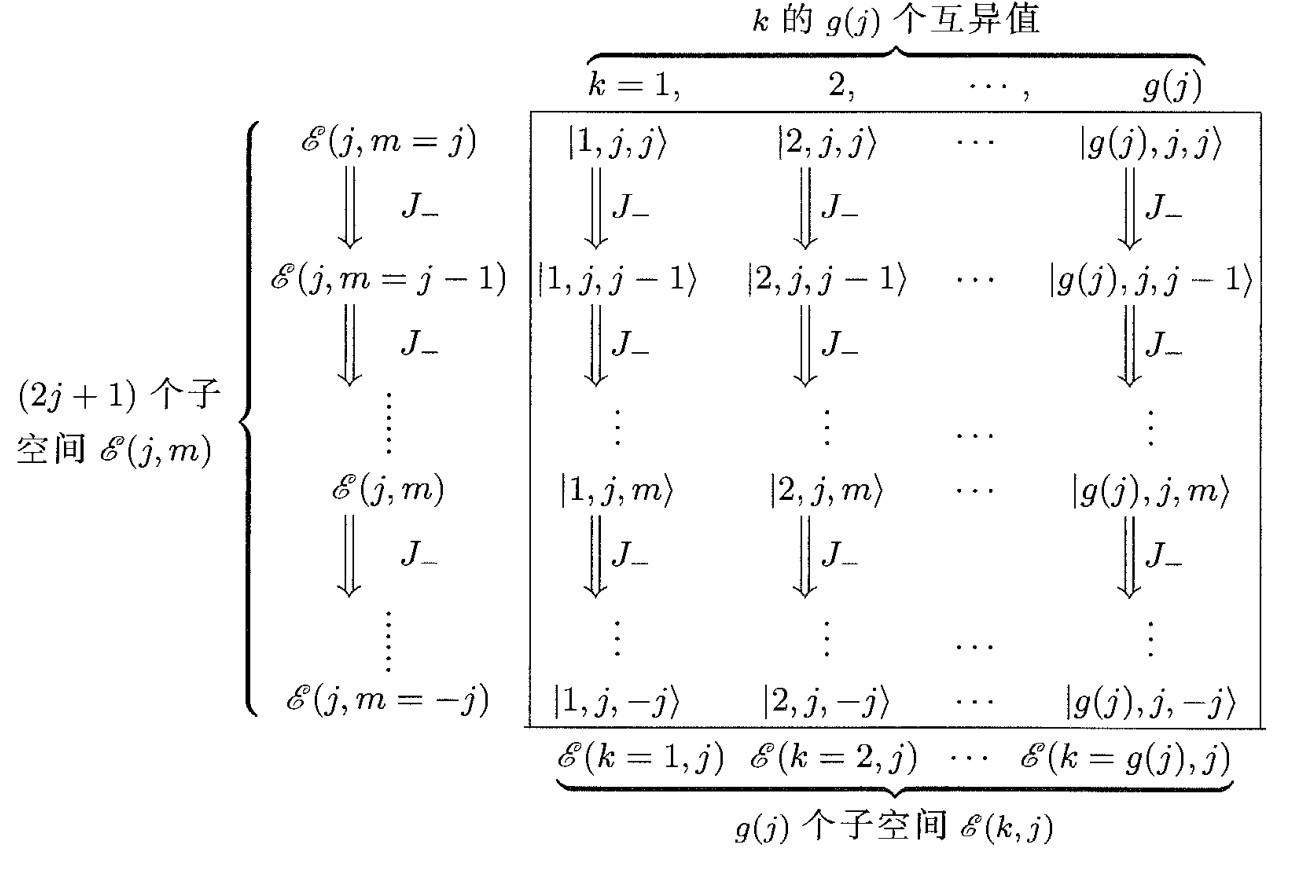
\includegraphics[width=0.9\textwidth]{figure/stadbasis.jpg}
            \caption{标准表象$|k,j,m\rangle$的生成}
            \label{fig5:standbasis}
        \end{figure}
        
        有两点值得注意的地方。首先,我们希望能用算符$\hat{A}$,使得$\hat{A},\hat{J^2},\hat{J_z}$构成态空间上的ESCO。同时,我们更希望升降算符作用以后的态仍然能够用算符$\hat{A}$来辨认,于是在这里我们需要一个额外的条件,即:$[\hat{J},\hat{A}]=0$\footnote{即算符$\hat{A}$是一个标量算符。这个想法是自然的}。
        
        其次,本节的讨论是基于$\mathcal{E}(j,m)$来构造整个态空间的正交归一基,但是在实际操作中有几个缺陷:
        \begin{enumerate}
            \item $\mathcal{E}(j,m)$的维数并不是事先知道的,与体系的性质有关系;
            \item 由于$\langle k_i,j,m|\hat{J_-}\hat{J_+}|k_s,j,m\rangle$一般不等于0,因此我们可以推出$\hat{J}|k,j,m\rangle \notin \mathcal{E}(j,m)$,即空间$\mathcal{E}(j,m)$在$\hat{J}$的作用下并不是不变的,这一点性质尤其不好。
        \end{enumerate}
        
        上述在实际操作中带来不便的因素促使我们思考另一种子空间的构造方法,即$\mathcal{E}(k,j)$。根据图\ref{fig5:standbasis}可知$\mathcal{E}(k,j)$的组成,经过简单演算我们可以知道以下两点:
        \begin{enumerate}
            \item $\mathcal{E}(k,j)$的简并度永远不变,等于$2j+1$
            \item $\mathcal{E}(k,j)$在$\hat{J},\hat{J^2},F(\hat{J})$下都保持不变
        \end{enumerate}
        
        本节我们只是简单的对总体情况做一个说明,在后面的内容中(尤其是对角动量的耦合以及氢原子的讨论),我们会有更多的实例来佐证本节的观点。
\section{自旋}\label{section5:spin}
    \subsection{自旋的实验引入}
    
    
    \subsection{$\frac{1}{2}$自旋态的表示}
        在上节的最后,我们提到了自旋角动量只与粒子本身的内禀属性有关。事实上,自旋角动量是一个相对论效应,Dirac通过建立Dirac方程可以来描述电子的自旋。由于本笔记在不说明的情况下都是仅仅讨论非相对论的量子力学,因此在本节中,我们采用Pauli的理论,通过加入一些假设使得自旋自洽的融入其中。
        
        由于电子的自旋是一个新的自由度,并且对于电子,我们可以通过量子电动力学证明$s=\frac{1}{2}$,则$m_s=\frac{\hbar}{2},-\frac{\hbar}{2}$。于是我们认为电子状态波函数是一个二分量的列旋量\footnote{这里注意,电子状态波函数构成的不是二分量的列矢量,因为自旋空间上的运动会影响位形空间 上的运动}。
        \begin{equation}
            |\psi(r,s_z,t)\rangle=\binom{\psi_1(r,t)}{\psi_2(r,t)}=\psi_1(r,t)|\alpha \rangle+\psi_2(r,t)|\beta\rangle
        \end{equation}
        
        其中我们认为$|\alpha\rangle$是自旋向上的,$|\beta\rangle$是自旋向下的,并且定义$|\alpha\rangle=\binom{1}{0},|\beta\rangle=\binom{0}{1}$。如果体系的$Hamiltonian$不含自旋角动量,或者自旋部分和空间部分可以分开\footnote{即$\hat{H}=\hat{H_s}+\hat{H_r}$},那么自旋态与位形空间上的态就可以分离:
        \begin{align}
            \begin{split}
                |\psi(r,s_z,t)\rangle=|\varphi(r,t)\rangle|\xi(s_z,t)\rangle\\
                |\xi(s_z,t)\rangle=\binom{\xi_1(t)}{\xi_2(t)}=\xi_1(t)|\alpha\rangle+\xi_2(t)|\beta \rangle
            \end{split}
        \end{align}
        
        于是在考虑自旋角动量后,我们可以将Schrodinger方程改写为两分量的方程,我们称之为Pauli方程。
        
        
        在\ref{section5.3.1}中,我们已经得到了角动量的一般理论,现在我们将其应用于自旋中,可以得到自旋角动量算符的对易关系和本征方程:
        \begin{align}
            \begin{split}
             [\hat{S_x},\hat{S_y}]=&i\hbar\hat{S_z}\\
             [\hat{S_x},\hat{S_y}]=&i\hbar\hat{S_z}\\
             [\hat{S_x},\hat{S_y}]=&i\hbar\hat{S_z}\\
            [\hat{S^2},\hat{S_i}]=0,i=&x,y,z\\
            \hat{S^2}|\psi\rangle=s(s+1)\hbar&|\psi\rangle\\
            \hat{S_z}|\psi\rangle=m_s\hbar|\psi\rangle,m_s=&s,s-1,\ldots,-s+1,-s
            \end{split}
        \end{align}
        
       由于自旋波函数是一个两分量的列旋量,因此自旋角动量分量算符$\hat{S_i}$一定可以表示成$2\times 2$的Hermite矩阵\footnote{下文讲述的只是自旋矩阵的一种常用表象,即Pauli表象而已,事实上我们并不能完全确定矩阵的具体性质,但是我们可以证明这三个矩阵一定是自逆,反对易,零迹的,详见张永德《量子力学》(第四版),科学出版社,p176-p179}。同时,由于态空间可以表示为自旋空间和位形空间的直积($\mathcal{E}=\mathcal{E}_r\otimes\mathcal{E}_s$),因此与自旋角动量有关的算符(如$\hat{S_z}$)可以作为$\mathcal{E}_s$空间上的延申算符。如果我们进一步假设$\hat{S_z}$的本征态是非简并的,于是我们有以下关系:
        \begin{align}
            \begin{split}
                \hat{S_z}|\alpha\rangle=&\frac{1}{2}\hbar|\alpha \rangle\\
                \hat{S_z}|\beta \rangle=&-\frac{1}{2}\hbar|\beta \rangle
            \end{split}
        \end{align}
        
        其中,由于$|\alpha \rangle,|\beta \rangle$是正交归一的,因此我们可以将$\{|\alpha \rangle,|\beta \rangle \}$看作自旋空间$\mathcal{E}_s$的基\footnote{这句话是显然的,但是由于概念比较重要,故在此多重复几遍},于是$\hat{S_z}$的矩阵形式为:
        \begin{equation}
        \hat{S_z}=\frac{\hbar}{2}
            \begin{pmatrix}
            1 & 0\\
            0 & -1
            \end{pmatrix}
        \end{equation}
    
        下面继续讨论其他两个自旋角动量分量算符对应的矩阵形式。根据\ref{equ3:totangularmom},我们知道,对于自旋空间上的态,升降算符的作用可以表示为:
        \begin{equation}
            \hat{J_\pm}|s,m_s\rangle=\sqrt{s(s+1)-m_s(m_s\pm 1)}\hbar |s,m_s-1\rangle
        \end{equation}
        
        将$s=\frac{1}{2},m_s=\frac{1}{2},-\frac{1}{2}$代入,可得\footnote{在这里$|\alpha\rangle=|\frac{1}{2},\frac{1}{2}\rangle,|\beta\rangle=|\frac{1}{2},-\frac{1}{2}\rangle$}:
        \begin{align}
            \begin{split}
                \hat{S_+}|\alpha\rangle=\hat{S_-}|\beta\rangle=0\\
                \hat{S_+}|\beta\rangle=\hbar |\alpha\rangle\\
                \hat{S_-}|\alpha\rangle=\hbar |\beta \rangle
            \end{split}
        \end{align}
        
        于是我们得到升降算符的矩阵形式:
        \begin{equation}
        \hat{S_+}=\hbar 
            \begin{pmatrix}
            1 & 0\\
            0 & 0
            \end{pmatrix}
        \end{equation}
        
        \begin{equation}
         \hat{S_-}=\hbar 
            \begin{pmatrix}
            0 & 0\\
            0 & 1
            \end{pmatrix}
        \end{equation}
        
        联立升降算符定义:$\hat{J_\pm}=\hat{J_+}\pm \hat{J_-}$和角动量算符分量算符的对易关系:$[\hat{S_x},\hat{S_y}]=i\hbar\hat{S_z}$,并且利用角动量分量算符是Hermite的,我们可以得到角动量分量算符的矩阵形式\footnote{再次重复,这里得到的矩阵形式只是$\{\hat{S_i}\}$的一种表象,被称为Pauli表象,实际上矩阵的形式是不确定的。在这里Pauli表象有两个约定:1、$\hat{S_z}$是对角的(或者等价说法是本征态是非简并的);2、$\hat{S_x}$的相位为0。显然,不同的表象之间利用某个$2\times2$的幺正变换矩阵相互联系}:
          \begin{equation}
        \hat{S_z}=\frac{\hbar}{2}
            \begin{pmatrix}
            1 & 0\\
            0 & -1
            \end{pmatrix}
        \end{equation}
          \begin{equation}
        \hat{S_x}=\frac{\hbar}{2}
            \begin{pmatrix}
            0 & 1\\
            -1 & 0
            \end{pmatrix}
        \end{equation}
          \begin{equation}
        \hat{S_y}=\frac{\hbar}{2}
            \begin{pmatrix}
            0 & -i\\
            i & 0
            \end{pmatrix}
        \end{equation}
       
       我们可以简记为$\hat{S_i}=\frac{\hbar}{2}\hat{\sigma_i}$,其中$\hat{\sigma_i}$被称作Pauli矩阵。由于$\hat{\sigma_x},\hat{\sigma_y},\hat{\sigma_z}\textrm{和单位矩阵}\hat{\sigma_0}$在$2\times2$复矩阵空间中是线性无关的,并且该空间的维数为4,因此$\hat{\sigma_x},\hat{\sigma_y},\hat{\sigma_z},\hat{\sigma_0}$一定构成$2\times2$复矩阵空间的一组基;也就是说,任意一个$2\times2$复矩阵都能表示成$\hat{\sigma_x},\hat{\sigma_y},\hat{\sigma_z},\hat{\sigma_0}$的线性组合\footnote{注意这里的展开系数是复数}。由于Pauli矩阵具有自逆,反对易性,零迹,为展开后的计算提供了便利。
\section{角动量的耦合}\label{section5:coupling}
    \subsection{为什么要讨论角动量的耦合?}\label{subsection5:coupling}
    本节我们简单讨论一下角动量的耦合给我们计算和处理问题带来了哪些便利,首先还是考虑经典力学模型。对于N个粒子的体系,给定原点O的总角动量可以表示成各粒子角动量之和:
    \begin{equation}
        L=\sum_{i=1}^{N}L_i
    \end{equation}
    
    其中$L_i=r_i\times p_i$。在经典力学中,一个重要的思考方式就是讨论各个物理量对时间的导数。如果导数为0,则称这个物理量为运动产量(或守恒量)。由于总角动量对时间的导数等于各个粒子对O点的力矩之和:
    \begin{equation}
        \frac{dL}{dt}=\sum_{i=1}^{N}M_i
    \end{equation}
    
    如果每个粒子不受外力(即$F_{i,external}=0$),或者每个粒子的力指向同一中心,则$dL/dt=0$,总角动量是运动常量。重要的点在于,总角动量是运动常量并不能代表每个粒子的角动量也是运动常量,如果每个粒子间存在相互作用,那么粒子间的内力会引起角动量的“传递”。
    
    现在考虑量子体系。假设有两个无相互作用、无自旋的粒子,它们的总$Hamiltonian$可以表示为$\hat{H}=\hat{H_1}+\hat{H_2}$,其中:
    \begin{align}
        \begin{split}
            \hat{H_1}=-\frac{\hbar^2}{2\mu_1}\nabla^2+\hat{V}(r_1)\\
            \hat{H_2}=-\frac{\hbar^2}{2\mu_2}\nabla^2+\hat{V}(r_2)
        \end{split}
    \end{align}
    
    我们可以从中计算出:
    \begin{equation}
        [\hat{L_1},\hat{H}]=[\hat{L_2},\hat{H}]=0
    \end{equation}
    
    因此如果粒子之间没有相互作用,那么它们的角动量算符都是运动常量。但是如果两个粒子之间存在相互作用\footnote{此处假设相互作用是保守力,即对应的势能只和$|r_1-r_2|$有关},此时总$Hamiltonian$可以表示为:$\hat{H}=\hat{H_1}+\hat{H_2}+\hat{V}(|r_1-r_2|)$。此时粒子的角动量就不是运动常量了,因为:
    \begin{equation}
        [\hat{L_1},\hat{H}]=[\hat{L_1},\hat{V}(|r_1-r_2|)]
    \end{equation}
    
    上式一般不等于0,比如我们可以取$L_1$的一个分量进行计算:
    \begin{align}
            [\hat{L_{1z},\hat{H}}]=[\hat{L_{1z}},\hat{V}(|r_1-r_2|)]
            =\frac{\hbar}{i}[\hat{x_1}\frac{\partial \hat{V}}{\partial \hat{y_1}}-\hat{y_1}\frac{\partial \hat{V}}{\partial \hat{x_1}}]
    \end{align}
    
    上式一般不等于0。但是如果考虑总角动量$\hat{L}=\hat{L_1}+\hat{L_2}$,那么可以验证总角动量就是运动常量:
    \begin{align}
        \begin{split}
            [\hat{L_z},\hat{H}]=&[\hat{L_{1z}}+\hat{L_{2z}}]\\
            =&\frac{\hbar}{i}[\hat{x_1}\frac{\partial \hat{V}}{\partial \hat{y_1}}-\hat{y_1}\frac{\partial \hat{V}}{\partial \hat{x_1}}+\hat{x_2}\frac{\partial \hat{V}}{\partial \hat{y_2}}-\hat{y_2}\frac{\partial \hat{V}}{\partial \hat{x_2}}]\\
            =&\frac{\hbar}{i}\frac{\hat{V'}}{|r_1-r_2|}[\hat{x_1}(\hat{y_1}-\hat{y_2})-\hat{y_1}(\hat{x_1}-\hat{x_2})+\hat{x_2}(\hat{y_2}-\hat{y_1})-\hat{y_2}(\hat{x_2}-\hat{x_1})]\\
            =&0
        \end{split}
    \end{align}
    
    其中:
    \begin{align}
        \begin{split}
            \frac{\partial \hat{V}}{\partial \hat{y_1}}=&\frac{\partial V}{\partial|r_1-r_2|}\frac{\partial|r_1-r_2|}{\partial y_1}\\
            =&V'\frac{\partial \Big((x_1-x_2)^2+(y_1-y_2)^2+(z_1-z_2)^2\Big)^{\frac{1}{2}} }{y_1}\\
            =&\frac{V'(y_1-y_2)}{|r_1-r_2|}
        \end{split}
    \end{align}
    
    同理:
    \begin{align}
        \begin{split}
            \frac{\partial \hat{V}}{\partial \hat{y_2}}=&\frac{V'(y_2-y_1)}{|r_1-r_2|}\\
            \frac{\partial \hat{V}}{\partial \hat{x_1}}=&\frac{V'(x_1-x_2)}{|r_1-r_2|}\\
            \frac{\partial \hat{V}}{\partial \hat{x_2}}=&\frac{V'(x_2-x_1)}{|r_1-r_2|}
        \end{split}
    \end{align}
    
    由此,我们得到了与经典力学相似的结论:当存在相互作用时,每个粒子的角动量与$Hamiltonian$不对易,因此体系不存在$\hat{L_i^2},\hat{L_{iz}},\hat{H}$的共同本征态来描述体系;但是由于总角动量算符是运动常量,因此我们能够用$\hat{L^2},\hat{L_z},\hat{H}$的共同本征态描述体系以得到体系的能量。
    
    最后我们简单的说明一下受到中心势场作用并且考虑自旋的粒子。此时我们可以利用微扰论证明,总$Hamiltonian$会出现一个微扰项(被称为自旋-轨道耦合项):$\hat{H_s}=
    \xi(r)\hat{L}\cdot \hat{S}$,这一项的出现导致了轨道角动量$\hat{L}$和自旋角动量$\hat{S}$都与$\hat{H}$不对易。此时我们考虑总角动量算符$\hat{J}=\hat{L}+\hat{S}$,此时有关系:
    \begin{align}
        \begin{split}
            [\hat{J_z},\hat{H}]=&[\hat{L_z}+\hat{S_z},
            \hat{H_s}]\\
            =&[\hat{L_z}+\hat{S_z},
            \xi(r)(\hat{L_x}\hat{S_x}+\hat{L_y}\hat{S_y}+\hat{L_z}\hat{S_z})]\\
            =&\xi(r)\Big([\hat{L_z},
            \hat{L_x}\hat{S_x}+\hat{L_y}\hat{S_y}+\hat{L_z}\hat{S_z}]+[\hat{S_z},
           \hat{L_x}\hat{S_x}+\hat{L_y}\hat{S_y}+\hat{L_z}\hat{S_z}]\Big)\\
            =&\xi(r)\Big( [\hat{L_z},\hat{L_x}]\hat{S_x}+\hat{L_x}[\hat{L_z},\hat{S_x}]+[\hat{L_z},\hat{L_y}]\hat{S_y}+\hat{L_y}[\hat{L_z},\hat{S_y}] \Big)\\
            =&\xi(r)\{-\hat{L_x}\hat{S_y}+\hat{L_y}\hat{S_x}+\hat{L_x}\hat{S_y}-\hat{L_y}\hat{S_x} \}\\
            =&0
        \end{split}
    \end{align}
    
    于是对于一般情况$\hat{J}=\hat{J_1}+\hat{J_2}$,总$Hamiltonian$对应的矩阵可以在一组新的基$\{\hat{J^2},\hat{J_z}\}$下被对角化。在本章的最后一节中,我们将会讨论$\{\hat{J_1^2},\hat{J_1z}\hat{J_2^2},\hat{J_{2z}}\} \textrm{到}\{ \hat{J_1^2},\hat{J^2}\hat{J_2^2},\hat{J_z}\}$的变换。
    
    
    \subsection{自旋-自旋耦合}
    本节考虑角动量耦合中最简单的情况,即两个自旋$\frac{1}{2}$粒子之间相互作用导致的自旋-自旋耦合关系(比如氢原子中的质子与电子),以此为基础来讨论一般角动量的耦合问题。由于每个粒子都有自旋向上和自旋向下两种不同的选择,因此两个粒子之间的自旋组合应该有4种\footnote{这里的自旋组合的写法是张量积的简记:$|a\rangle\otimes|A\rangle\rightarrow|a\rangle|A\rangle$}:$|a\rangle|A\rangle,|a\rangle|B\rangle,|b\rangle|A\rangle,|b\rangle|B\rangle$。其中大小写字母代表不同的粒子,$|a\rangle,|A\rangle$代表自旋向上,$|b\rangle,|B\rangle$代表自旋向下。根据上节的内容,我们需要考虑总自旋算符$\hat{S}$
    \begin{equation}
        \hat{S}=\hat{S_1}+\hat{S_2}
    \end{equation}
    
    那么对于$\hat{S_1},\hat{S_2}$的本征态$|\xi_1\rangle,|\xi_2\rangle$,我们根据张量积的关系可以得到$|\hat{S}\rangle$对应的本征方程:
    \begin{align}
        \begin{split}
            \hat{S_z}|\xi_1\rangle|\xi_2\rangle=&(\hat{S_{1z}}+\hat{S_{2z}})|\xi_1\rangle|\xi_2\rangle\\
        =&(\widehat{S_{1z}}|\xi_1\rangle)|\xi_2\rangle+|\xi_1\rangle(\widehat{S_{2z}}|\xi_2\rangle)\\
        =&(m_1+m_2)\hbar|\xi_1\rangle|\xi_2\rangle\\
        =& m_s\hbar|\xi_1\rangle|\xi_2\rangle
        \end{split}
    \end{align}
 
 由上式我们知道,两粒子体系角动量算符$\hat{S_z}$的本征值是两个粒子可能本征值的相加,因此对于4种粒子自旋的组合,其$m_s$有三种情况:$m_s=1,0,-1$,下面我们分别讨论这三种情况。
 
 在\ref{subsection5:coupling}节中,我们知道,在本节中,我们的目标是讨论映射:$\{\widehat{S_1^2},\widehat{S_2^2},\widehat{S_1z},\widehat{S_2z}\}\rightarrow\{\widehat{S_1^2}\widehat{S_2^2},\widehat{S^2},\widehat{S_z}\}$,即构造态$|s,m_s\rangle$,将其表示成$|s_1,s_2\rangle$的线性组合\footnote{由于在latex中打分数太烦了,于是下面统一用英文字母代表自旋向上向下}。在上面的讨论中,我们已经知道$\hat{S_z}$算符的本征方程了,现在我们讨论$\hat{S^2}$的作用,对于$|a\rangle|A\rangle$\footnote{下式成立的一个重要前提就是不同粒子的角动量算符一定是对易的,即$[\hat{S_1},\hat{S_2}]=0$}。(即$m_s=1$的情况) 
 \begin{align}
  \begin{split}
      \hat{S^2}|a\rangle|A\rangle=&(\hat{S_1^2}+\hat{S_2^2}+\hat{S_1}\hat{S_2}+\hat{S_2}\hat{S_1})|a\rangle|A\rangle\\
      =&(\hat{S_1^2}+\hat{S_2^2}+2\hat{S_1}\cdot \hat{S_2})|a\rangle|A\rangle\\ 
      =&\Bigl(\hat{S_1^2}+\hat{S_2^2}+2(\widehat{S_{1x}} \widehat{S_{2x}}+\widehat{S_{1y}} \widehat{S_{2y}}+\widehat{S_{1z}} \widehat{S_{2z}})\Bigr)|a\rangle|A\rangle\\
      =&2\hbar^2|a\rangle|A\rangle
  \end{split} 
 \end{align}

其中:
\begin{align}
    (\hat{S_1^2}+\hat{S_2^2})|a\rangle|A\rangle=(\hat{S_1^2}|a\rangle)|A\rangle+|a\rangle(\hat{S_2^2}|A\rangle)=\frac{3}{2}\hbar^2|a\rangle|A\rangle
\end{align}
\begin{align}
    \begin{split}
        \widehat{S_{1x}}\widehat{S_{2x}}|a\rangle|A\rangle=&\widehat{S_{1x}}|a\rangle \otimes \widehat{S_{2x}}|A\rangle\\
        =&\frac{1}{2}\hbar \begin{pmatrix}
        0 & 1\\
        1 & 0
        \end{pmatrix}\binom{1}{0}\otimes \frac{1}{2}\hbar \begin{pmatrix}
        0 & 1\\
        1 & 0
        \end{pmatrix}\binom{1}{0}\\
        =&\frac{1}{2}\hbar\binom{0}{1}\otimes \frac{1}{2}\hbar\binom{0}{1}\\
        =&\frac{\hbar^2}{4}|b\rangle|B\rangle
    \end{split}
\end{align}
\begin{align}
    \begin{split}
        \widehat{S_{1y}}\widehat{S_{2y}}|a\rangle|A\rangle=&\widehat{S_{1y}}|a\rangle \otimes \widehat{S_{2y}}|A\rangle\\
        =&\frac{1}{2}\hbar \begin{pmatrix}
        0 & -i\\
        i & 0
        \end{pmatrix}\binom{1}{0}\otimes \frac{1}{2}\hbar \frac{1}{2}\hbar \begin{pmatrix}
        0 & -i\\
        i & 0
        \end{pmatrix}\binom{1}{0}\\
        =&\frac{1}{2}\hbar\cdot i\cdot \binom{0}{1}\otimes \frac{1}{2}\hbar\cdot i \cdot \binom{0}{1}\\
        =&-\frac{\hbar^2}{4}|b\rangle|B\rangle
    \end{split}
\end{align}
\begin{align}
    \begin{split}
        \widehat{S_{1z}}\widehat{S_{2z}}|a\rangle|A\rangle=&\widehat{S_{1z}}|a\rangle \otimes \widehat{S_{2z}}|A\rangle\\
        =&\frac{1}{2}\hbar \begin{pmatrix}
        1 & 0\\
        0 & -1
        \end{pmatrix}\binom{1}{0}\otimes \frac{1}{2}\hbar \begin{pmatrix}
        1 & 0\\
        0 & -1
        \end{pmatrix}\binom{1}{0}\\
        =&\frac{1}{2}\hbar\binom{1}{0}\otimes \frac{1}{2}\hbar\binom{1}{0}\\
        =&\frac{\hbar^2}{4}|a\rangle|A\rangle
    \end{split}
\end{align}

当$m_s=-1$,也就是考虑$|b\rangle|B\rangle$态的时候,我们可以验证情况是类似的:
\begin{equation}
    \hat{S^2}|b\rangle|B\rangle=2\hbar^2|b\rangle|B\rangle
\end{equation}

于是我们有:
\begin{align}
    \begin{split}
        |1,1\rangle=|a\rangle|A\rangle\\
        |1,-1\rangle=|b\rangle|B\rangle
    \end{split}
\end{align}

当$m_s=0$时,情况稍有不同:
 \begin{align}\label{equ5:A}
  \begin{split}
      \hat{S^2}|a\rangle|B\rangle=&(\hat{S_1^2}+\hat{S_2^2}+\hat{S_1}\hat{S_2}+\hat{S_2}\hat{S_1})|a\rangle|B\rangle\\
      =&(\hat{S_1^2}+\hat{S_2^2}+2\hat{S_1}\cdot \hat{S_2})|a\rangle|B\rangle\\ 
      =&\Bigl(\hat{S_1^2}+\hat{S_2^2}+2(\widehat{S_{1x}} \widehat{S_{2x}}+\widehat{S_{1y}} \widehat{S_{2y}}+\widehat{S_{1z}} \widehat{S_{2z}})\Bigr)|a\rangle|B\rangle\\
      =&\frac{3}{2}\hbar^2|a\rangle|B\rangle+\hbar^2|b\rangle|A\rangle-\frac{\hbar^2}{2}|a\rangle|B\rangle\\
      =&\hbar^2(|a\rangle|B\rangle+|b\rangle|A\rangle)
  \end{split} 
 \end{align}
 
 其中:
 \begin{align}
    (\hat{S_1^2}+\hat{S_2^2})|a\rangle|B\rangle=(\hat{S_1^2}|a\rangle)|B\rangle+|a\rangle(\hat{S_2^2}|B\rangle)=\frac{3}{2}\hbar^2|a\rangle|B\rangle
\end{align}
\begin{align}
    \begin{split}
        \widehat{S_{1x}}\widehat{S_{2x}}|a\rangle|B\rangle=&\hat{S_{1x}}|a\rangle \otimes \widehat{S_{2x}}|B\rangle\\
        =&\frac{1}{2}\hbar \begin{pmatrix}
        0 & 1\\
        1 & 0
        \end{pmatrix}\binom{1}{0}\otimes \frac{1}{2}\hbar \begin{pmatrix}
        0 & 1\\
        1 & 0
        \end{pmatrix}\binom{0}{1}\\
        =&\frac{1}{2}\hbar\binom{0}{1}\otimes \frac{1}{2}\hbar\binom{1}{0}\\
        =&\frac{\hbar^2}{4}|b\rangle|A\rangle
    \end{split}
\end{align}
\begin{align}
    \begin{split}
        \widehat{S_{1y}}\widehat{S_{2y}}|a\rangle|B\rangle=&\hat{S_{1y}}|a\rangle \otimes \widehat{S_{2y}}|B\rangle\\
        =&\frac{1}{2}\hbar \begin{pmatrix}
        0 & -i\\
        i & 0
        \end{pmatrix}\binom{1}{0}\otimes \frac{1}{2}\hbar  \begin{pmatrix}
        0 & -i\\
        i & 0
        \end{pmatrix}\binom{0}{1}\\
        =&\frac{1}{2}\hbar\cdot (-i)\cdot \binom{0}{1}\otimes \frac{1}{2}\hbar\cdot i \cdot \binom{1}{0}\\
        =&\frac{\hbar^2}{4}|b\rangle|A\rangle
    \end{split}
\end{align}
\begin{align}
    \begin{split}
        \widehat{S_{1z}}\widehat{S_{2z}}|a\rangle|A\rangle=&\hat{S_{1z}}|a\rangle \otimes \widehat{S_{2z}}|A\rangle\\
        =&\frac{1}{2}\hbar \begin{pmatrix}
        1 & 0\\
        0 & -1
        \end{pmatrix}\binom{1}{0}\otimes \frac{1}{2}\hbar \begin{pmatrix}
        1 & 0\\
        0 & -1
        \end{pmatrix}\binom{0}{1}\\
        =&\frac{1}{2}\hbar\binom{1}{0}\otimes \frac{1}{2}\cdot (-1)\cdot \hbar\binom{0}{1}\\
        =&-\frac{\hbar^2}{4}|a\rangle|B\rangle
    \end{split}
\end{align}

同理,我们可以验证:
\begin{equation}\label{equ5:B}
    \hat{S^2}|b\rangle|A\rangle=\hbar^2(|a\rangle|B\rangle+|b\rangle|A\rangle)
\end{equation}

由式\eqref{equ5:A}和\eqref{equ5:B},我们可以发现,两式中同时出现了$|a\rangle|B\rangle,|b
\rangle|A\rangle$,因此不能作为算符$\hat{S^2}$的本征方程。我们的目标是构造两个耦合态,从而构造算符$\hat{S^2}$的本征方程;换句话说,对于算符$\hat{S^2}$,其在基$|a\rangle|B\rangle,|b\rangle|A\rangle$下对应的矩阵形式为$\hbar^2\left(
\begin{smallmatrix} 1 & 1\\ 1 & 1
\end{smallmatrix}\right)$,并不是对角矩阵,我们的目的是将其对角化,得到在$|s,m_s\rangle$下的本征值与本征态。按照线性代数的知识,我们先求出$m_s=0$的自旋子空间的本征态:
\begin{equation}
    \begin{vmatrix}
    \hbar^2-\lambda & \hbar^2\\
    \hbar^2 & \hbar^2-\lambda 
    \end{vmatrix}=0 \rightarrow \lambda=2\hbar^2 \quad\textrm{or}\quad 0
\end{equation}

当$\lambda=2\hbar^2$时,代入行列式可以求出本征态为\footnote{注意这里还要考虑归一化的问题}:
\begin{equation}
    |1,0\rangle=\frac{1}{\sqrt{2}}(|a\rangle|B\rangle+|b\rangle|A\rangle)
\end{equation}

而当$\lambda=0$时,代入行列式可以求出本征态为:
\begin{equation}
    |0,0\rangle=\frac{1}{\sqrt{2}}(|a\rangle|B\rangle-|b\rangle|A\rangle)
\end{equation}

我们用线性代数的语言重新总结一下上述内容:我们的目标是将$|s,m_s\rangle$表示成$|s_1,s_2\rangle$的线性组合,构造出$\hat{S^2},\hat{S_z}$的本征方程。对于$\hat{S_z}$来说,我们可以证明其本征值为两个粒子的$\hat{S_{iz}}$的本征值之和;对于$\hat{S^2}$来说,在$m_s=0$的子空间中相互耦合的方程组导致我们无法直接得到本征方程,需要先对矩阵对角化。对角化的结果是产生两个耦合态。综上所述,$|s,m_s\rangle$的表示如下\footnote{在这里恢复了$|s_1,s_2\rangle$符号的记述,请自行与前文的符号对应}:
\begin{align}
    \begin{split}
        |1,-1\rangle=&|-\frac{1}{2},-\frac{1}{2}\rangle\\
        |1,0\rangle=&\frac{1}{\sqrt{2}}\Bigl(|\frac{1}{2},-\frac{1}{2}\rangle+|-\frac{1}{2},\frac{1}{2}\rangle\Bigr)\\
        |1,1\rangle=&|\frac{1}{2},\frac{1}{2}\rangle\\
        |0,0\rangle=&\frac{1}{\sqrt{2}}\Bigl(|\frac{1}{2},-\frac{1}{2}\rangle-|-\frac{1}{2},\frac{1}{2}\rangle\Bigr)
    \end{split}
\end{align}

前三个耦合态对应$\hat{S_z}\textrm{的本征值为}2\hbar^2$的情况,称为三重态,可以简单验证,它们是自旋对称的;$|0,0\rangle$对应$\hat{S_z}\textrm{的本征值为}0$的情况,称为单态,可以简单验证,它们是自旋反对称的。我们将会在第\ref{chapter:identicalparticles}章中展示这个结论的重要意义。
    \subsection{一般角动量的耦合}
        \subsubsection{基本概念复习}
        本节我们根据上节的求解的内容出发,希望得到一般的两个角动量的耦合特点。我们首先复习一下必要的内容。对于两粒子体系来说,每个粒子的角动量算符分别为$\hat{J_1},\hat{J_2}$,对应的态空间为$\mathcal{E}_1,\mathcal{E}_2$,根据\ref{subsubsection5:standardbasis}节的内容,我们一定可以在$\mathcal{E}_1,\mathcal{E}_2$上分别取标准表象$\{|k_1,j_1,m_1\rangle,|k_2,j_2,m_2\rangle\}$,并且满足以下关系;
     \begin{align}
         \begin{split}
            \hat{J_1^2}|k_1,j_1,m_1\rangle= j_1(j_1+1)\hbar^2|k_1,j_1,m_1\rangle\\
            \hat{J_2^2}|k_2,j_2,m_2\rangle= j_2(j_2+1)\hbar^2|k_2,j_2,m_2\rangle
         \end{split}
     \end{align}
     \begin{align}
         \begin{split}
            \widehat{J_{1z}}|k_1,j_1,m_1\rangle=m_1\hbar|k_1,j_1,m_1\rangle\\
            \widehat{J_{2z}}|k_2,j_2,m_2\rangle= m_2\hbar|k_2,j_2,m_2\rangle
         \end{split}
     \end{align}
     \begin{align}
         \begin{split}
            \widehat{J_{1\pm}}|k_1,j_1,m_1\rangle =\sqrt{j_1(j_1+1)- m_1(m_1\pm1)}\hbar|k_1,j_1,m_1\pm1\rangle\\
             \widehat{J_{2\pm}}|k_2,j_2,m_2\rangle =\sqrt{j_2(j_2+1)- m_2(m_2\pm1)}\hbar|k_2,j_2,m_2\pm1\rangle 
         \end{split}
     \end{align}
    
    体系总的态空间可以表示为两个粒子态空间的张量积:$\mathcal{E}=\mathcal{E}_1\otimes\mathcal{E}_2$。如果我们选定$\mathcal{E}_1\textrm{和}\mathcal{E}_2$上的标准表象$\{|k_1,j_1,m_1\rangle\},\{|k_2,j_2,m_2\rangle\}$,那么$\{|k_1,j_1,m_1\rangle\}\otimes\{|k_2,j_2,m_2\rangle\}$一定是$\mathcal{E}$上的一组正交归一基,我们将其记作$|k_1,k_2;j_1,j_2;m_1,m_2\rangle$。
    
    根据\ref{subsubsection5:standardbasis}节的内容,如果我们从子空间的角度上来分析,我们可以将$\mathcal{E}_1,\mathcal{E}_2$空间看成标准表象下若干子空间的直和:
    \begin{align}
    \begin{split}
        \mathcal{E}_1=&\sum_{\oplus}\mathcal{E}(k_1,j_1)\\
         \mathcal{E}_2=&\sum_{\oplus}\mathcal{E}(k_2,j_2)
    \end{split}
    \end{align}
    
    于是$\mathcal{E}$可以表示为:
    \begin{equation}
        \mathcal{E}=\sum_{\oplus}\mathcal{E}(k_1,k_2;j_1,j_2)=\sum_{\oplus}\mathcal{E}(k_1,j_1)\otimes\mathcal{E}(k_2,j_2)
    \end{equation}
    
    其中$\mathcal{E}(k_1,k_2;j_1,j_2)$的维数为$(2j_1+1)(2j_2+1)$。并且有一个重要的性质,即这个空间对于$\hat{J_1},\hat{J_2}$\footnote{严格来说,这里的$\hat{J_1},\hat{J_2}$是其在对应的$\mathcal{E}_1$上的延伸算符}的任意函数的作用保持不变。这是后续讨论最重要的基础。
    \subsubsection{问题的提出}
    根据\ref{subsection5:coupling}节最后所说,我们的最终目标是讨论$\{\hat{J_1^2},\hat{J_2^2},\widehat{J_{1z}},\widehat{J_{2z}}\}\rightarrow \{\hat{J_1^2},\hat{J_2^2},\hat{J},\hat{J_z}\}$。首先验证$\{\hat{J_1^2},\hat{J_2^2},\hat{J},\hat{J_z}\}$是否构成$\mathcal{E}$上的ESCO。
    
    对于总角动量算符$\hat{J}=\hat{J_1}+\hat{J_2}$,其平方算符一定可以表示为:
    \begin{equation}
        \hat{J^2}=\hat{J_1^2}+\hat{J_2^2}+2\hat{J_1}\cdot\hat{J_2}
    \end{equation}
    
    因此经过简单验证,我们可以得到以下对易关系:
    \begin{align}\label{equ5:coupling_commutive}
        \begin{split}
            [\hat{J^2},\hat{J_1}]=[\hat{J^2},\hat{J_2}]=0\\
            [\hat{J^2},\hat{J_1^2}]=[\hat{J^2},\hat{J_2^2}]=0\\
            [\hat{J_z},\widehat{J_{1z}}]=[\hat{J_z},\widehat{J_{1z}}]=0
        \end{split}
    \end{align}
    
    值得注意的是,由于$\hat{J^2}\textrm{含有}\hat{J_1},\hat{J_2}$的耦合项,因此$\hat{J^2}\textrm{与}\widehat{J_{1z}},\widehat{J_{2z}}$不对易。根据ESCO的定义,同时我们需要考虑态空间最小长度的ESCO,因此我们只能选择相互对易的四个算符$\{\hat{J_1^2},\hat{J_2^2},\hat{J},\hat{J_z}\}$构成$\mathcal{E}$上的ESCO。
    
    第二个问题是$\{\hat{J_1^2},\hat{J_2^2},\widehat{J_{1z}},\widehat{J_{2z}}\}$ 通过怎样的基变换得到$ \{\hat{J_1^2},\hat{J_2^2},\hat{J},\hat{J_z}\}$。根据上节的内容,我们知道态空间$\mathcal{E}(j_1,j_2)$\footnote{由于$\mathcal{E}(k_1,k_2,j_1,j_2)\textrm{中}F(\hat{J})$的矩阵元与$k_1,k_2$无关,因此只要$j_1,j_2$相同,矩阵的对角化是完全相同的,故我们可以将$\mathcal{E}(k_1,k_2;j_1,j_2)$简写为$\mathcal{E}(j_1,j_2)$;同时态空间内的标准表象$|k_1,k_2;j_1,j_2;m_1,m_2\rangle$可以简写为$|j_1,j_2;m_1,m_2\rangle$}在$F(\hat{J_1}),F(\hat{J_2})$中保持不变,因此$\mathcal{E}(j_1,j_2)$也一定在$F(\hat{J})$下保持不变\footnote{可以那么理解:$F(\hat{J})=F(\hat{J_1}+\hat{J_2})=F'(\hat{J_1},\hat{J_2})$。也就是说,我们总可以由$\hat{J_1}\textrm{和}\hat{J_2}$的任意函数形式组成$\hat{J}$的某个函数}。换句话说$\hat{J^2},\hat{J_z}$在基$\{\hat{J_1^2},\hat{J_2^2},\widehat{J_{1z}}\}$所对应的矩阵在$\mathcal{E}(j_1,j_2)$空间中有非零矩阵元,由此我们将态空间$\mathcal{E}$上的基变换问题转化为了子空间$\mathcal{E}(j_1,j_2)$上的基变换问题,具体有如下两个问题:
    \begin{enumerate}
        \item 由于$\mathcal{E}(j_1,j_2)$在$F(\hat{J})$的作用下保持不变,因此按照$j$的取值不同,我们一定可以将$\mathcal{E}(j_1,j_2)$表示成不同j值对应子空间的直和:
        \begin{equation}
            \mathcal{E}(j_1,j_2)=\sum_{\oplus}\mathcal{E}(k,j)
        \end{equation}
        那么$j$的取值如何?
        \item $\mathcal{E}(j_1,j_2)$的本征态如何在$|j_1,j_2;m_1,m_2\rangle$下展开成$|j,m
        \rangle$?
    \end{enumerate}
    
    我们也可以这样理解,考虑本征方程:
    \begin{align}
        \begin{split}
            \hat{J^2}|k,j,m\rangle=&j(j+1)\hbar^2|k,j,m\rangle\\
            \hat{J_z}|k,j,m\rangle=&m\hbar|k,j,m\rangle
        \end{split}
    \end{align}
    
    在求解本征方程的过程中,我们需要两组关系:$j,m\textrm{与}j_1,m_1;j_2,m_2$之间的关系以及$|j_1,j_2,j,m\rangle$和$|j_1,j_2;m_1,m_2\rangle$之间的关系。
    
    \subsubsection{问题的解决}
    我们首先考虑$\hat{J_z}$的本征值,根据式\eqref{equ5:coupling_commutive}中的$ [\hat{J_z},\widehat{J_{1z}}]=[\hat{J_z},\widehat{J_{1z}}]=0$,我们知道$\hat{J_z},\widehat{J_{1z}},\widehat{J_{2z}}$能够拥有一组共同本征矢,记作$\{|m,m_1,m_2\rangle\}$,于是一定有关系:
    \begin{align}
    \begin{split}
         m\hbar|m,m_1,m_2\rangle=&\hat{J_z}|m,m_1,m_2\rangle\\
         =&(\widehat{J_{1z}}+\widehat{J_{2z}})|m,m_1,m_2\rangle\\
         =&(m_1+m_2)\hbar|m,m_1,m_2\rangle
    \end{split}
    \end{align}
    于是:
    \begin{equation}
        m=m_1+m_2
    \end{equation}
    我们知道对于角动量算符来说$m$的取值为$j,j-1,\cdots,-j+1,-j$,由此我们可以发现磁量子数的最大值一定等于总角动量的最大值,即:
    \begin{equation}
        j_{max}=j_{1max}+j_{2max}=m_1+m_2
    \end{equation}
    
    并且取值一定是依次减1的,现在问题只剩下$j$的最小取值了,根据上文的讨论,我们知道对于态空间$\mathcal{E}(j_1,j_2)$,由于其定义为两个空间$\mathcal{E}(j_1,m_1),\mathcal{E}(j_2,m_2)$的直积,因此其维数为$(2j_1+1)(2j_2+1)$;同时$\mathcal{E}(j_1,j_2)$可以按照$j$的取值进行划分:
    \begin{equation}
        \mathcal{E}(j_1+j_2)=\mathcal{E}_{j_1+j_2}\oplus\mathcal{E}_{j_1+j_2-1}\oplus\cdots \oplus \mathcal{E}_{j_{min}}
    \end{equation}
    
    对于子空间$\mathcal{E}_j$来说,其维数为$2j+1$,于是有以下维数的恒等式:
   \begin{equation}
        (2j_1+1)(2j_2+1)=\big(2(j_1+j_2)+1\big)+\big(2(j_1+j_2-1)+1\big)+\cdots +(2j_{min}+1)
   \end{equation}
    
    展开可得:
    \begin{align}
    \begin{split}
        4j_1j_2+2j_1+2j_2+1=&\sum_{j=j_{min}}^{j_1+j_2}2j+1\\
         =& 2\cdot \sum_{j=j_{min}}^{j_1+j_2}j+\sum_{j=j_{min}}^{j_1+j_2}1\\
         =& 2\cdot \frac{(j_{min}+j_1+j_2)(j_1+j_2-j_{min}+1)}{2}\\
         &+(j_1+j_2-j_{min}+1)\\
         =& (j_{min}+j_1+j_2)(j_1+j_2-j_{min}+1)\\
         &+(j_1+j_2-j_{min}+1)\\
         =& (j_1+j_2-j_{min}+1)(j_1+j_2+j_{min}+1)\\
         =& (j_1+j_2+1)^2-j_{min}^2\\
         \Longrightarrow j_{min}^2=&(j_1+j_2+1)^2-2j_1j_2-2j_1-2j_2-1\\
         =& (j_1-j_2)^2\\
         \Longrightarrow j_{min}=& |j_1-j_2|
    \end{split}
    \end{align}
    
    因此,一旦$j_1,j_2$给定,则一定有$m=m_1+m_2$,$j$的取值为$j_1+j_2,j_1+j_2-1,\cdots,|j_1-j_2|$,同时态空间$\mathcal{E}(j_1,j_2)$存在两种分解形式:
    \begin{align}
    \begin{split}
         \mathcal{E}(j_1,j_2)=&\mathcal{E}(j_1,m_1)\otimes\mathcal{E}(j_2,m_2)\\
         =&\mathcal{E}_{j_1+j_2}\oplus\mathcal{E}_{j_1+j_2-1}\oplus\cdots \oplus \mathcal{E}_{|j_1-j_2|}
    \end{split}
    \end{align}

上式是角动量的耦合的核心思想,下面我们讨论如何用$|j_1,j_2,j,m\rangle$表示$|j_1,j_2,m_1,m_2\rangle$。我们首先通过一个比自旋-自旋耦合稍难的例子入手求解上述问题,然后通过类比给出一般方法。

现在我们考虑$j_1=1,j_2=\frac{1}{2}$时角动量的耦合情况。首先我们验证一下两种分解方法是否维数相等。根据上面的讨论,我们知道$j$的取值只有两种,即:$j=\frac{3}{2},\frac{1}{2}$。根据$j$的取值,我们知道,当$j=\frac{3}{2}$时,$m=\frac{3}{2},\frac{1}{2},-\frac{1}{2},-\frac{3}{2}$,由此可知$\mathcal{E}_{j_{max}}=\mathcal{E}_{j=\frac{3}{2}}$是一个四维空间;当$j=\frac{1}{2}$时,$m=\frac{1}{2},-\frac{1}{2}$,由此可知$\mathcal{E}_{j_{max}}=\mathcal{E}_{j=\frac{1}{2}}$是一个二维空间。因此$\mathcal{E}(j_1,j_2)=\mathcal{E}(1,\frac{1}{2})$是一个六维空间。同时,当$j_1=1$时,$m_1=1,0,-1$,因此$\mathcal{E}(j_1,m_1)$的维数为3;同理,当$j_2=\frac{1}{2}$时,$\mathcal{E}(j_2,m_2)$的维数为2,因此两者的张量积空间维数为6。于是我们就验证了两种分解态空间的等价性。

在前面的内容中,我们已经知道,由于$j_{max}=j_{1max}+j_{2max}=m_1+m_2=m$这个限制条件,因此对于$j=m$的情况下,$|j_1,j_2,j,m\rangle\textrm{与}|j_1,j_2,m_1,m_2\rangle$是完全等价的,由此,我们能够通过$|\frac{3}{2},\frac{3}{2}\rangle=|1,\frac{1}{2}\rangle$与升降算符的作用得到其他用$|m_1,m_2\rangle$表示$|j,m\rangle$\footnote{由于拥有相同的$j_1,j_2$,因此$|j_1,j_2,j,m\rangle$可以简写为$j,m\rangle$;$|j_1,j_2,m_1,m_2\rangle$可以简写为$|m_1,m_2\rangle$}的表达式,具体如下:
\begin{align}
    \begin{split}
        \sqrt{j(j+1)-m(m-1)}\hbar|\frac{3}{2},\frac{1}{2}\rangle=&\hat{J_-}|\frac{3}{2},\frac{3}{2}\rangle\\
        =&(\widehat{J_{1z}}+\widehat{J_{2z}})|1,\frac{1}{2}\rangle\\
        =&\sqrt{j_1(j_1+1)-m_1(m_1-1)}\hbar|0,\frac{1}{2}\rangle\\
        &+\sqrt{j_2(j_2+1)-m_2(m_2-1)}\hbar|1,-\frac{1}{2}\rangle
    \end{split}
\end{align}

代入$j=\frac{3}{2},m=\frac{3}{2};j_1=1,m_1=1;j_2=\frac{1}{2},m_2=\frac{1}{2}$,可得:
\begin{equation}\label{equ5:down}
    |\frac{3}{2},\frac{1}{2}\rangle=\sqrt{\frac{2}{3}}|0,\frac{1}{2}\rangle+\sqrt{\frac{1}{3}}|1,-\frac{1}{2}\rangle
\end{equation}

由此我们得到了$|\frac{3}{2},\frac{1}{2}\rangle$被对应的$|m_1,m_2\rangle$---$|0,\frac{1}{2}\rangle$和$|1,-\frac{1}{2}\rangle$线性表示的式子,利用下降算符继续作用于$|\frac{3}{2},\frac{1}{2}\rangle$上,并重复上述过程。最后,我们可以得到$j=\frac{3}{2}$的全部4个态矢量:$|\frac{3}{2},\frac{3}{2}\rangle,|\frac{3}{2},\frac{1}{2}\rangle,|\frac{3}{2},-\frac{1}{2}\rangle,|\frac{3}{2},-\frac{3}{2}\rangle$被对应的$|m_1,m_2\rangle$线性表示的表达式。

下面考虑$j=\frac{1}{2}$时的情况,相比上面一种情况困难的地方在于,此时没有$|j,m\rangle=|m_1,m_2\rangle$的情况。但是我们知道,对于任意一个$|j,m\rangle$态,我们一定可以写成满足条件的$|m_1,m_2\rangle$态的线性组合。于是对于$|\frac{1}{2},\frac{1}{2}\rangle$态来说,我们一定可以写成:
\begin{equation}
    |\frac{1}{2},\frac{1}{2}\rangle=a|1,-\frac{1}{2}\rangle+b|0,\frac{1}{2}\rangle
\end{equation}
由于不同子空间上的态是相互正交的,于是一定有关系:
\begin{equation}
    \langle \frac{3}{2},\frac{1}{2}|\frac{1}{2},\frac{1}{2}\rangle=0
\end{equation}

将式\eqref{equ5:down}代入,并且根据归一化条件:$a^2+b^2=1$,可得:$a=\sqrt{\frac{1}{3}},b=-\sqrt{\frac{2}{3}}$。随后利用下降算符作用于$|\frac{1}{2},\frac{1}{2}\rangle$,利用与$j=\frac{3}{2}$类似的方法可以得到$|\frac{1}{2},-\frac{1}{2}\rangle$。于是,我们就求解了$j_1=1,j_2=\frac{1}{2}$的所有情况

对于任意的$j_1,j_2$,情况是类似的,方法如下:
\begin{itemize}
    \item 对于每一个符合要求的$|j,m\rangle$态,一定可以表示成满足$m=m_1+m_2$的所有态$|m_1,m_2\rangle$的线性组合。其中有一种特别的情况,当$m=j_{max}=j_1+j_2$时,此时满足$m=m_1+m_2$的情况只有一种,即$m_1=j_1;m_2=j_2$。于是此时$|j,m\rangle=|m_1,m_2\rangle$,这是非常关键的等式。
    \item 由于我们讨论问题在标准表象$|k,j,m\rangle$下,因此我们采用升降算符构造态空间$\mathcal{E}(j_1,j_2)$上我们需要的标准表象$|j_1,j_2,j,m\rangle$。首先考虑子空间$\mathcal{E}_{j_{max}}$,此时由于$m=j_{max}=j_1+j_2$的时候$|j,m\rangle=|m_1,m_2\rangle$,我们在等号两边同时作用下降算符,并取对应空间上的延伸算符即可以得到$|j_1+j_2,j_1+j_2-1\rangle$被$|j_1-1,j_2\rangle$和$|j_1,j_2-1\rangle$线性表示。具体说来,则有:
    \begin{align}
        \begin{split}
            \sqrt{2(j_1+j_2)}\hbar|j_1+j_2,j_1+j_2-1\rangle=&\hat{J_{-}}|j_1+j_2,j_1+j_2\rangle\\
            =&(\widehat{J_{1z}}+\widehat{J_{2z}})|j_1,j_2\rangle\\
            =&\sqrt{2j_1}\hbar|j_1-1,j_2\rangle+\sqrt{2j_2}\hbar|j_1,j_2-1\rangle
        \end{split}
    \end{align}
    
    由此可得:
    \begin{equation}
        |j_1+j_2,j_1+j_2-1\rangle=\sqrt{\frac{j_1}{j_1+j_2}}|j_1-1,j_2\rangle+\sqrt{\frac{j_2}{j_1+j_2}}|j_1,j_2-1\rangle
    \end{equation}

    用下降算符继续作用,重复上述操作即可以得到$\mathcal{E}_{j_1+j_2}$所有的基底$|j,m\rangle$。
    \item 下面考虑其他子空间$\mathcal{E}_j$,我们首先从$\mathcal{E}_{j_1+j_2}$的补空间的子空间中$j$的最大值$j=j_1+j_2-1$所在的子空间开始讨论。同样,由于$m=m_1+m_2$的限制,对于态矢量$|j_1+j_2-1\rangle,j_1+j_2-1\rangle$来说,我们可以将其看成满足条件的$|m_1,m_2\rangle$的线性组合:
    \begin{equation}
        |j_1+j_2-1\rangle,j_1+j_2-1\rangle=a|j_1,j_2-1\rangle+b|j_1-1,j_2\rangle
    \end{equation}
    
    为了解出$a,b$,按照例子中的思路,我们讨论其与$\mathcal{E}_{j_1+j_2}$中任意一个基的标量积为0:(当然,实际操作中,为了计算方便,我们往往选择$|j_1+j_2,j_1+j_2-1\rangle$)
    \begin{equation}
        \langle j_1+j_2,j_1+j_2-1|j_1+j_2-1,j_1+j_2-1\rangle=
        \sqrt{\frac{j_1}{j_1+j_2}}a+\sqrt{\frac{j_2}{j_1+j_2}}b=0
    \end{equation}
   
    同时,根据归一化条件$a^2+b^2=1$,我们可以解出$a=-\sqrt{\frac{j_2}{j_1+j_2}},b=\sqrt{\frac{j_1}{j_1+j_2}}$,从而得到:
    \begin{equation}
        |j_1+j_2-1\rangle,j_1+j_2-1\rangle=-\sqrt{\frac{j_2}{j_1+j_2}}|j_1,j_2-1\rangle+\sqrt{\frac{j_1}{j_1+j_2}}|j_1-1,j_2\rangle
    \end{equation}
    
    随后我们通过下降算符构造$\mathcal{E}_{j_1+j_2-1}$的所有基底$|j,m\rangle$。
    \item 我们重复上面步骤,取$\mathcal{E}_{j_1+j_2}\oplus\mathcal{E}_{j_1+j_2-1}$的补空间中$j$的最大值$j=j_1+j_2-2$,考虑满足$j_1+j_2-2=m=m_1+m_2$的线性组合,随后通过与不同空间基的正交性与态的归一化得到线性组合的系数,最后利用下降算符获得$\mathcal{E}_{j_1+j_2-2}$的所有基底,以此类推$\cdots$
\end{itemize}

由此,我们就将所有的$|j,m\rangle$用对应的$|m_1,m_2\rangle$线性表示,用通式表示为:
\begin{equation}
    |j,m\rangle=\sum_{m_1=-j_1}^{j_1}\sum_{m_2=-j_2}^{j_2}\langle m_1,m_2|j,m\rangle\cdot |m_1,m_2\rangle
\end{equation}

其中,我们称系数$\langle m_1,m_2|j,m\rangle$为Clebsch-Gordan系数,我们可以通过查表得方式获得确定得$j_1,j_2$下得C-G系数,详见图\ref{fig5:CGcoefficient}:
\begin{figure}[H]
    \centering
    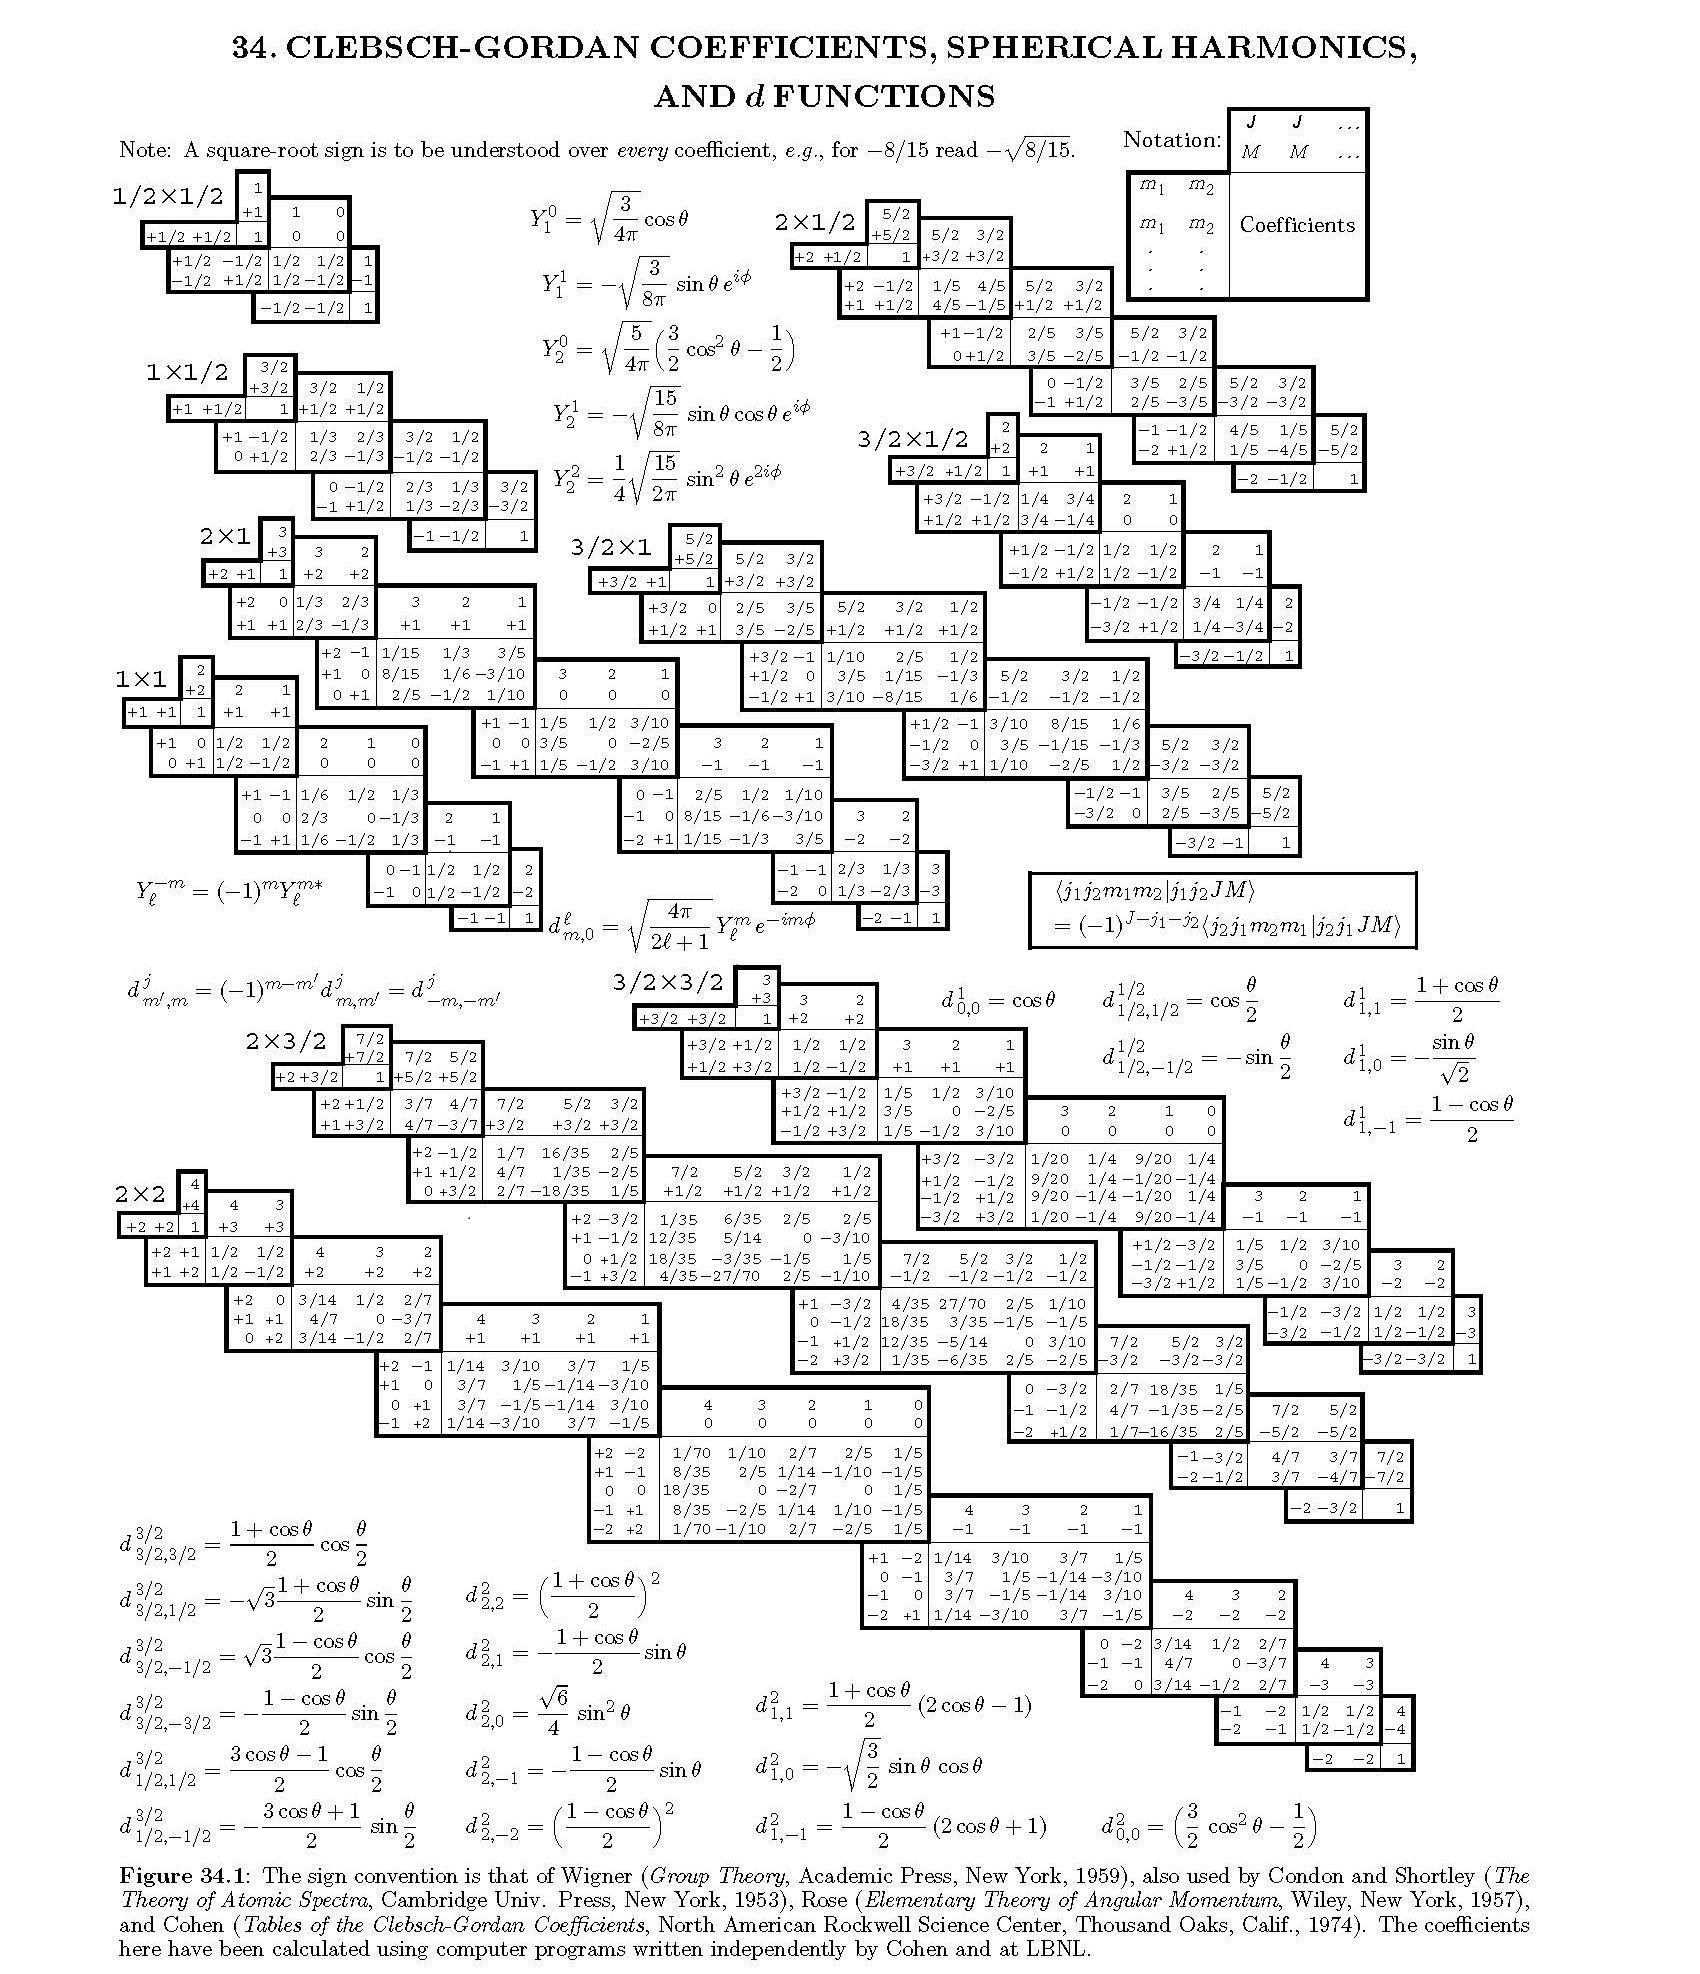
\includegraphics[width=\textwidth]{figure/CGcoefficent.jpg}
    \caption{C-G系数表}
    \label{fig5:CGcoefficient}
\end{figure}
